\documentclass[12pt]{article}
\usepackage[left=1cm, right=1cm, top=2cm,bottom=1.5cm]{geometry} 

\usepackage[parfill]{parskip}
\usepackage[utf8]{inputenc}
\usepackage[T2A]{fontenc}
\usepackage[russian]{babel}
\usepackage{enumitem}
\usepackage[normalem]{ulem}
\usepackage{amsfonts, amsmath, amsthm, amssymb, mathtools,xcolor,accents}
\usepackage{blkarray}

\usepackage{tabularx}
\usepackage{hhline}

\usepackage{accents}
\usepackage{fancyhdr}
\pagestyle{fancy}
\renewcommand{\headrulewidth}{1.5pt}
\renewcommand{\footrulewidth}{1pt}

\usepackage{graphicx}
\usepackage[figurename=Рис.]{caption}
\usepackage{subcaption}
\usepackage{float}

%%Наименование папки откуда забирать изображения
\graphicspath{ {./images/} }

%%Изменение формата для ввода доказательства
\renewcommand{\proofname}{$\square$  \nopunct}
\renewcommand\qedsymbol{$\blacksquare$}

%%Изменение отступа на таблицах
\addto\captionsrussian{%
	\renewcommand{\proofname}{$\square$ \nopunct}%
}
%% Римские цифры
\newcommand{\RN}[1]{%
	\textup{\uppercase\expandafter{\romannumeral#1}}%
}

%% Для удобства записи
\newcommand{\MR}{\mathbb{R}}
\newcommand{\MC}{\mathbb{C}}
\newcommand{\MQ}{\mathbb{Q}}
\newcommand{\MN}{\mathbb{N}}
\newcommand{\MZ}{\mathbb{Z}}
\newcommand{\MTB}{\mathbb{T}}
\newcommand{\MTI}{\mathbb{I}}
\newcommand{\MI}{\mathrm{I}}
\newcommand{\MCI}{\mathcal{I}}
\newcommand{\MJ}{\mathrm{J}}
\newcommand{\MH}{\mathrm{H}}
\newcommand{\MT}{\mathrm{T}}
\newcommand{\MU}{\mathcal{U}}
\newcommand{\MV}{\mathcal{V}}
\newcommand{\MA}{\mathcal{A}}
\newcommand{\MB}{\mathcal{B}}
\newcommand{\MF}{\mathcal{F}}
\newcommand{\ME}{\mathcal{E}}
\newcommand{\MW}{\mathcal{W}}
\newcommand{\ML}{\mathcal{L}}
\newcommand{\MP}{\mathcal{P}}
\newcommand{\VN}{\varnothing}
\newcommand{\VE}{\varepsilon}
\newcommand{\dx}{\, dx}
\newcommand{\dy}{\, dy}
\newcommand{\dz}{\, dz}
\newcommand{\dd}{\, d}


\theoremstyle{definition}
\newtheorem{defn}{Опр:}
\newtheorem{rem}{Rm:}
\newtheorem{prop}{Утв.}
\newtheorem{exrc}{Упр.}
\newtheorem{problem}{Задача}
\newtheorem{lemma}{Лемма}
\newtheorem{theorem}{Теорема}
\newtheorem{corollary}{Следствие}

\newenvironment{cusdefn}[1]
{\renewcommand\thedefn{#1}\defn}
{\enddefn}

\DeclareRobustCommand{\divby}{%
	\mathrel{\text{\vbox{\baselineskip.65ex\lineskiplimit0pt\hbox{.}\hbox{.}\hbox{.}}}}%
}
\DeclareRobustCommand{\ndivby}{\mkern-1mu\not\mathrel{\mkern4.5mu\divby}\mkern1mu}


%Короткий минус
\DeclareMathSymbol{\SMN}{\mathbin}{AMSa}{"39}
%Длинная шапка
\newcommand{\overbar}[1]{\mkern 1.5mu\overline{\mkern-1.5mu#1\mkern-1.5mu}\mkern 1.5mu}
%Функция знака
\DeclareMathOperator{\sgn}{sgn}

%Функция ранга
\DeclareMathOperator{\rk}{\text{rk}}
\DeclareMathOperator{\diam}{\text{diam}}


%Обозначение константы
\DeclareMathOperator{\const}{\text{const}}

\DeclareMathOperator{\codim}{\text{codim}}

\DeclareMathOperator*{\dsum}{\displaystyle\sum}
\newcommand{\ddsum}[2]{\displaystyle\sum\limits_{#1}^{#2}}
\newcommand{\ddssum}[2]{\displaystyle\smashoperator{\sum\limits_{#1}^{#2}}}
\newcommand{\ddlsum}[2]{\displaystyle\smashoperator[l]{\sum\limits_{#1}^{#2}}}
\newcommand{\ddrsum}[2]{\displaystyle\smashoperator[r]{\sum\limits_{#1}^{#2}}}

%Интеграл в большом формате
\DeclareMathOperator{\dint}{\displaystyle\int}
\newcommand{\ddint}[2]{\displaystyle\int\limits_{#1}^{#2}}
\newcommand{\ssum}[1]{\displaystyle \sum\limits_{n=1}^{\infty}{#1}_n}

\newcommand{\smallerrel}[1]{\mathrel{\mathpalette\smallerrelaux{#1}}}
\newcommand{\smallerrelaux}[2]{\raisebox{.1ex}{\scalebox{.75}{$#1#2$}}}

\newcommand{\smallin}{\smallerrel{\in}}
\newcommand{\smallnotin}{\smallerrel{\notin}}

\newcommand*{\medcap}{\mathbin{\scalebox{1.25}{\ensuremath{\cap}}}}%
\newcommand*{\medcup}{\mathbin{\scalebox{1.25}{\ensuremath{\cup}}}}%

\makeatletter
\newcommand{\vast}{\bBigg@{3.5}}
\newcommand{\Vast}{\bBigg@{5}}
\makeatother

%Промежуточное значение для sup\inf, поскольку они имеют разную высоту
\newcommand{\newsup}{\mathop{\smash{\mathrm{sup}}}}
\newcommand{\newinf}{\mathop{\mathrm{inf}\vphantom{\mathrm{sup}}}}

%Скалярное произведение
\newcommand{\inner}[2]{\left\langle #1, #2 \right\rangle }
\newcommand{\linsp}[1]{\left\langle #1 \right\rangle }
\newcommand{\linmer}[2]{\left\langle #1 \vert #2\right\rangle }

%Подпись символов снизу
\newcommand{\ubar}[1]{\underaccent{\bar}{#1}}

%%Шапка для букв сверху
\newcommand{\wte}[1]{\widetilde{#1}}
\newcommand{\wht}[1]{\widehat{#1}}
\newcommand{\ovl}[1]{\overline{#1}}


%%Трансформация Фурье
\newcommand{\fourt}[1]{\mathcal{F}\left(#1\right)}
\newcommand{\ifourt}[1]{\mathcal{F}^{-1}\left(#1\right)}

%%Символ вектора
\newcommand{\vecm}[1]{\overrightarrow{#1\,}}

%%Пространстов матриц
\newcommand{\matsq}[1]{\operatorname{Mat}_{#1}}
\newcommand{\mat}[2]{\operatorname{Mat}_{#1, #2}}

%Оператор для действ и мнимых чисел
\DeclareMathOperator{\IM}{\operatorname{Im}}
\DeclareMathOperator{\RE}{\operatorname{Re}}
\DeclareMathOperator{\li}{\operatorname{li}}
\DeclareMathOperator{\GL}{\operatorname{GL}}
\DeclareMathOperator{\SL}{\operatorname{SL}}
\DeclareMathOperator{\Char}{\operatorname{char}}
\DeclareMathOperator\Arg{Arg}
\DeclareMathOperator\ord{ord}

%Оператор для образа
\DeclareMathOperator{\Ima}{Im}

%Делимость чисел
\newcommand{\modn}[3]{#1 \equiv #2 \; (\bmod \; #3)}
\newcommand{\nmodn}[3]{#1 \not\equiv #2 \; (\bmod \; #3)}

%%Взятие в скобки, модули и норму
\newcommand{\parfit}[1]{\left( #1 \right)}
\newcommand{\modfit}[1]{\left| #1 \right|}
\newcommand{\sqparfit}[1]{\left\{ #1 \right\}}
\newcommand{\normfit}[1]{\left\| #1 \right\|}

%%Функция для обозначения равномерной сходимости по множеству
\newcommand{\uconv}[1]{\overset{#1}{\rightrightarrows}}
\newcommand{\uconvm}[2]{\overset{#1}{\underset{#2}{\rightrightarrows}}}

%% Функция для добавления круга сверху множества
\newcommand{\Circ}[1]{\accentset{\circ}{#1}}

%%Функция для обозначения нижнего и верхнего интегралов
\def\upint{\mathchoice%
	{\mkern13mu\overline{\vphantom{\intop}\mkern7mu}\mkern-20mu}%
	{\mkern7mu\overline{\vphantom{\intop}\mkern7mu}\mkern-14mu}%
	{\mkern7mu\overline{\vphantom{\intop}\mkern7mu}\mkern-14mu}%
	{\mkern7mu\overline{\vphantom{\intop}\mkern7mu}\mkern-14mu}%
	\int}
\def\lowint{\mkern3mu\underline{\vphantom{\intop}\mkern7mu}\mkern-10mu\int}

%%След матрицы
\DeclareMathOperator*{\tr}{tr}

\makeatletter
\renewcommand*\env@matrix[1][*\c@MaxMatrixCols c]{%
	\hskip -\arraycolsep
	\let\@ifnextchar\new@ifnextchar
	\array{#1}}
\makeatother


%% Переопределение функции хи, чтобы выглядела более приятно
\makeatletter
\@ifdefinable\@latex@chi{\let\@latex@chi\chi}
\renewcommand*\chi{{\@latex@chi\smash[t]{\mathstrut}}} % want only bottom half of \mathstrut
\makeatletter

\setcounter{MaxMatrixCols}{20}

\begin{document}
\lhead{Математический анализ - \RN{4}}
\chead{Шапошников С.В.}
\rhead{Лекция - 13}
\section*{Меры Лебега}
\subsection*{Мера Лебега на $\MR^n$}

\begin{theorem}
	Пусть $L(x) = Ax + b, \, L \colon \MR^n \to \MR^n$, где $A \in \mat{n}{n}$, $b$ - вектор. Тогда для всякого измеримого ограниченного множества $E$ верно равенство:
	$$
		\lambda(L(E)) = |\det{A}|{\cdot}\lambda(E)
	$$
\end{theorem}
\begin{rem}
	Заметим, что: 
	$$
		|\det{A}| = \sqrt{\det{A}{\cdot}\det{A}} = \sqrt{\det{(A{\cdot}A)}} = \sqrt{\det{(A^TA)}} 
	$$ 
	Как найти элементы матрицы $A^TA$? Если $e_1, \dotsc, e_n$ это ортонормированный базис, то её столбцы можно находить так: $A^TAe_j$, но если есть скалярное произведение в пространстве, то можно выразить сам элемент матрицы (см. линейную алгебру):
	$$
		\inner{A^TAe_i}{e_j} = (A^TA)_{ij} = \inner{Ae_i}{Ae_j} \Rightarrow \MR^n_x \xrightarrow{y = Ax}\MR^n_y
	$$
	Следовательно, кубик, натянутый на $(e_1,\dotsc, e_n)$ в $\MR^n_x$, переходит в параллелепипед, натянутый на $(Ae_1, \dotsc, Ae_n)$ в $\MR_y^n$. Тогда $v_i = Ae_i$ - вектора на которые натянут определитель $A$ и $(\inner{v_i}{v_j})$ это матрица Грама. Таким образом:
	$$
		\lambda(L(E)) = \const{\cdot}\lambda(E) \Rightarrow \const = \sqrt{\det{(\inner{v_i}{v_j})}}
	$$
	где $\const$ вычисляется из того, что мы смотрим в какой параллелепипед переносится единичный куб и для этих векторов: $(v_1, \dotsc, v_n)$ считаем матрицу Грама. Такой вариант записи без изменения переносится на всякие плоскости в $\MR^n$ и без изменений переносится на кривые поверхности, когда $L$ уже перестает быть линейным отображением и $\lambda(L(E))$ это уже мера Хаусдорфа. В этом случае матрица Грама берется для векторов, соответствующих параллелепипеду - образу единичного куба при отображении, которое для общего отображения является его аффинным приближением по формуле Тейлора.
\end{rem}

\subsection*{Мера Лебега на $\MR^k$}

Пусть у нас есть $\MR^n$, $\inner{v}{u} = v_1u_1 + \dotsc + v_n u_n$ - фиксированы. Возьмем $\Pi_k \subset \MR^n$ - $k$-мерную аффинную плоскость и выбираем в ней прямоугольную систему координат: $(\eta_1,\dotsc, \eta_k), \, \inner{\eta_i}{\eta_j} = \delta_{ij}$ (то есть, с точки зрения фиксированного скалярного произведения это ортонормированные вектора) и тогда каждой точке сопоставляется набор из $(y_1,\dotsc, y_k)$. После такого сопоставления мы отождествляем $\Pi_k$ с $\MR^k$ и с $\MR^k$ переносим на $\Pi_k$ меру Лебега: $\lambda_{\Pi_k} \Rightarrow$ можем измерять $k$-мерные объемы.
\begin{theorem}
	$L(x) = Ax + b \colon \MR^k \to \MR^n$, где $n \geq k$ и $\rk{(A)} = k$. Тогда $L(\MR^k) = \Pi_k$ - $k$-мерная аффинная плоскость в $\MR^n$ и верно, что для всякого измеримого ограниченного множества $E \subset \MR^k$:
	$$
		\lambda_{\Pi_k}(L(E)) = \sqrt{\det{(A^T{\cdot}A)}}{\cdot}\lambda(E)
	$$
\end{theorem}
\begin{rem}
	У нас параметрическое задание плоскости в $\MR^3$ из аналитической геометрии. Например:
	$$
		L \colon \MR^2 \to \MR^3, \, L(x) = b + x_1\eta + x_2 \xi = b + A
		\begin{pmatrix}
			x_1 \\
			x_2
		\end{pmatrix}, \, \eta = Ae_1 = 
		\begin{pmatrix}
			\eta_1 \\
			\eta_2\\
			\eta_3
		\end{pmatrix}, \, \xi = Ae_2 =
		\begin{pmatrix}
			\xi_1 \\
			\xi_2\\
			\xi_3
		\end{pmatrix}, \, 
		b = \begin{pmatrix}
			b_1 \\
			b_2\\
			b_3
		\end{pmatrix}
	$$
\end{rem}
\begin{proof}
	Рассмотрим плоскость $\Pi_k \subset \MR^n$, которая задается так: $L(x) = Ax + b$, то есть к концу вектора $b$ прикладываются всевозможные вектора $Ax \Rightarrow$ получается $k$-мерная аффинная плоскость. Поместим в конец вектора $b$ прямоугольную систему координат: $(\eta_1,\dotsc, \eta_k), \, \inner{\eta_i}{\eta_j} = \delta_{ij}$. Тогда у каждой точки $\Pi_k$ появятся координаты, следовательно: $Ax \mapsto (y_1,\dotsc, y_k)$, где $y_j = \inner{Ax}{\eta_j}$. Получили отображение: 
	$$
		B \colon \MR_x^k \to \MR_y^k, \, B(x_1,\dotsc,x_k) = (\inner{Ax}{\eta_1}, \inner{Ax}{\eta_2}, \dotsc, \inner{Ax}{\eta_k}) = (y_1,y_2,\dotsc, y_k)
	$$
	Очевидно, что $B$ это линейное, невырожденное отображение, поскольку это просто смена системы координат (матрица перехода). Поскольку $\lambda_{\Pi_k}(L(E))$ это по определению ввод ортонормированной системы координат,  переписывание $L(E)$ в координатах $(y_1,\dotsc, y_k)$ и затем расчёт обычной меры Лебега, то:
	$$
		\lambda_{\Pi_k}(L(E)) = \lambda(B(E)) = |\det{B}|{\cdot}\lambda(E) = \sqrt{\det(B^TB)}{\cdot}\lambda(E) = \sqrt{\det(\inner{Be_i}{Be_j})}{\cdot}\lambda(E) 
	$$
	Рассмотрим матрицу $(\inner{Be_i}{Be_j})$, где $e_i, e_j \in \MR^k$. Матрица Грама устроена так:
	$$
		\inner{Be_i}{Be_j}_{\MR^k_y} = \ddsum{s}{}\inner{Ae_i}{\eta_s}_{\MR^n} {\cdot}\inner{Ae_j}{\eta_s}_{\MR^n} = \inner{Ae_i}{Ae_j}_{\MR^n} = \inner{A^TAe_i}{e_j}_{\MR^k_x} \Rightarrow |\det{B}| = \sqrt{\det(A^TA)}
	$$
	где мы использовали тот факт, что: 
	$$
		Be_s = B(0, \dotsc, 0, \underset{s}{1}, 0, \dotsc, 0) = (\inner{Ae_s}{\eta_1}, \inner{Ae_s}{\eta_2} \dotsc, \inner{Ae_s}{\eta_k}), \, s = i,j
	$$
	Остальные равенства проверяются непосредственным переходом к координатам, например:
	$$
		\inner{Ae_i}{\eta_s}_{\MR^n} = a_{1i}{\cdot}\eta_{1s} + a_{2i}{\cdot}\eta_{2s} + \dotsc + a_{ni}{\cdot}\eta_{ns} \Rightarrow 
	$$
	$$	
		\Rightarrow \inner{Ae_i}{\eta_s}_{\MR^n} {\cdot}\inner{Ae_j}{\eta_s}_{\MR^n} = a_{1i}{\cdot}a_{1j}{\cdot}\eta_{1s}^2 + a_{1i}{\cdot}a_{2j}{\cdot}\eta_{1s}{\cdot}\eta_{2s} + \dotsc + a_{ni}{\cdot}a_{nj}{\cdot}\eta_{ns}^2 + \dotsc
	$$
	$$
		\forall i = \ovl{1,n}, \, \ddsum{s = 1}{k}\eta_{is}^2 = 1 = \inner{\eta_i}{\eta_i}, \quad \forall i \neq j, \, \ddsum{s = 1}{k}\eta_{is}\eta_{js} = 0 = \inner{\eta_i}{\eta_j} \Rightarrow
	$$
	$$
		\Rightarrow  \ddsum{s}{}\inner{Ae_i}{\eta_s}_{\MR^n} {\cdot}\inner{Ae_j}{\eta_s}_{\MR^n} = a_{1i}{\cdot}a_{1j} + a_{2i}{\cdot}a_{2j} + \dotsc + a_{ni}{\cdot}a_{nj} = \inner{Ae_i}{Ae_j}_{\MR^n}
	$$
\end{proof}

\section*{Мера Хаусдорфа}
Пусть мы находимся в пространстве $\MR^n$.
\begin{defn}
	Пусть $0 < \alpha \leq n$, $\delta > 0$, тогда \uwave{вспомогательной мерой} называется функция:
	$$
		H_\delta^\alpha(E) = \inf\left\{\ddsum{j}{}(\diam{F_j})^\alpha \colon E \subset \cup_j F_j, \, F_j \text{ - замкнутые}, \, \diam{F_j} = \sup\limits_{x,y \in F_j} |x - y| \leq \delta \right\}
	$$
\end{defn}
Замкнутые множества берем, поскольку при замыкании диаметр не меняется и сумма не меняется также $\Rightarrow$ если умеем покрывать чем-то, то замыкаем и будем покрывать замкнутыми. При этом на точную нижнюю грань это не скажется никак. 

Заметим, что выше, при $\delta \to 0+$ у нас множество становится меньше $\Rightarrow$ точная нижняя грань может лишь только увеличиться $\Rightarrow$ возможно лишь невозрастание $H_\delta^\alpha(E) \Rightarrow$ функция монотонна.

\begin{defn}
	Функция: $H^\alpha(E) = \lim\limits_{\delta \to 0+} H_\delta^\alpha(E)$, где допустимо значение $+\infty$, называется \uwave{мерой Хаусдорфа}.
\end{defn}	

Сделаем ряд полезных наблюдений, когда мы обсуждаем меру Хаусдорфа.

\subsection*{Вычисление длины прямой мерой Хаусдорфа}
Пусть у нас есть отрезок длины $l$ и мы хотим метрически определить его длину. Возьмем покрытие отрезка в виде $\VE$-сети (отрезок - компакт $\Rightarrow$ конечное покрытие):
\begin{figure}[H]
	\centering
	\includegraphics[width=0.45\textwidth]{MA4L13_1.eps}
	\caption{Покрытие отрезка длины $l$ $\VE$-сетью.}
	\label{13_1}
\end{figure}
$N_{\VE}$ - количество $\VE$-шаров, покрывающих отрезок $\Rightarrow$ длина будет оцениваться, как $N_{\VE}{\cdot}2\VE$. Поскольку покрытие может быть каким угодно и можно покрывать одно и то же место по несколько раз, то естественно взять самое маленькое выражение: $\inf N_{\VE}{\cdot}2\VE$. Очевидно, что:
$$
	l \leq \inf N_{\VE}{\cdot}2\VE
$$
Можно покрывать отрезок дизъюнктно и выбрать покрытие так, чтобы было верно: 
$$
	N_\VE = \dfrac{l}{2\VE} \Rightarrow l \leq \inf N_{\VE}{\cdot}2\VE \leq N_{\VE}{\cdot}2\VE + 2\VE = l + 2\VE
$$ 
Далее мы сможем устремить $\VE \to 0$. Или подобрать покрытие так, чтобы: $l \leq \inf N_{\VE}{\cdot}2\VE \leq N_{\VE}{\cdot}2\VE = l$, поскольку для оценки снизу нам нужно любое покрытие, а для оценки сверху = какое-то. Тоже самое можно проделать с площадью: $\inf N_\VE {\cdot}\pi \VE^2$. По тем же самым соображениям будет получаться: 
$$
	S = \inf N_\VE {\cdot}\pi \VE^2
$$

Мера Хаусдорфа в данном случае хороша тем, что ровно таким же способом будем определять площади, длины и так далее, причем уже не важно, какой объект - любое множество будем накрывать любыми замкнутыми множествами (шары не всегда удобны для покрытия). 

После покрытия, посчитаем количество покрытий и умножим на диаметр в подходящей степени $\alpha$ (в зависимости от объекта, который хотим посчитать: длина $\Rightarrow \alpha = 1$, площадь $\Rightarrow \alpha = 2$, и так далее), затем будем брать точную нижнюю грань таких выражений: 
$$
	c{\cdot}l = \inf N_{\VE}{\cdot}(2\VE)^\alpha \Rightarrow \alpha = 1 \Rightarrow c{\cdot}l = \inf N_{\VE}{\cdot}(2\VE)
$$
В какой-то момент, окажется, что $\alpha$ может быть дробным. Покрытия не обязательно будут одинаковыми, допустим разные элементы покрытия.

\subsection*{Вычисление произвольной кривой мерой Хаусдорфа}
Хотелось бы понять, зачем нам нужно $\delta \to 0$, зачем двухступенчатое определение? Рассмотрим:
$$
	H^\alpha_*(E) = \inf\left\{\ddsum{j}{}(\diam{F_j})^\alpha \colon E \subset \cup_j F_j, \, F_j \text{ - замкнутые} \right\}
$$
Посчитаем длину единичной окружности. Есть замкнутое множество, которое эту окружность покрывает - сама окружность/круг, тогда $H^\alpha_*(E) \leq 2$, но при этом длина единичной окружности это $2\pi$. 
\begin{figure}[H]
	\centering
	\includegraphics[width=0.15\textwidth]{MA4L13_2.eps}
	\caption{Покрытие окружности одним кругом.}
	\label{13_2}
\end{figure}
Аналогично, если мы возьмем очень изрезанную кривую и не будем требовать, чтобы диаметры покрывающих множеств были маленькие, то мы не сможем поймать геометрическую структуру этой кривой, поскольку её можно будет накрыть одним множеством. 
\begin{figure}[H]
	\centering
	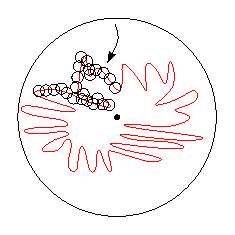
\includegraphics[width=0.15\textwidth]{MA4L13_3.eps}
	\caption{Измельчение $\delta$ позволяет учитывать геометрическую структуру.}
	\label{13_3}
\end{figure}
Если не будем мельчить покрытие, то никогда не поймаем изгибы, изрезанность или какие-либо другие структуры $\Rightarrow$ для этого приходится брать мельче покрытие $\Rightarrow$ получаем эффект, что уменьшая $\delta$ у нас начинает возрастать мера: двигаемся по всё более и более кривой дороге $\Rightarrow$ путь увеличивается.

\begin{prop}
	$H^\alpha$ - внешняя мера и все борелевские множества измеримы.
\end{prop}
\begin{proof}
	Проверим, что $H_\delta^\alpha$ это внешняя мера:
	\begin{enumerate}[label=\arabic*)]
		\item $\forall \delta > 0, \, \VN \subset F = \ovl{\MB}(0, \delta) \Rightarrow$ покрываем точкой $\Rightarrow \diam{F} = 0  \Rightarrow H_\delta^\alpha(\VN) = 0$;
		\item $A \subset B \Rightarrow \forall $ покрытия $B$ множествами $F_j, \, \diam{F_j} \leq \delta$ верно, что: 
		$$
			A \subset \cup_j F_j \Rightarrow H_\delta^\alpha(A) \leq \sum_j (\diam{F_j})^\alpha
		$$
		поскольку у нас точная нижняя грань в $H_\delta^\alpha(A)$. Заметим, что $ H_\delta^\alpha(A)$ это нижняя граница для $\sum_j (\diam{F_j})^\alpha$, а $H_\delta^\alpha(B)$ это точная нижняя граница, тогда по определению: $H_\delta^\alpha(A) \leq H_\delta^\alpha(B)$;
		\item Докажем полуаддитивность. Рассмотрим $\cup_m A_m$:
		$$
			\forall m, \, A_m \subset \bigcup\limits_j F_j^m \colon \diam{F_j^m} \leq \delta, \,  \sum_j( \diam{F_j^m})^\alpha \leq H_\delta^\alpha(A_m) + \dfrac{\VE}{2^m} \Rightarrow
		$$
		$$
			\Rightarrow \bigcup\limits_m A_m \subset \bigcup\limits_{m,j}F_j^m, \, \ddsum{m,j}{}(\diam{F_j^m})^\alpha \leq \ddsum{m}{}H_\delta^\alpha(A_m) + \VE \xrightarrow[\VE \to 0]{} \ddsum{m}{}H_\delta^\alpha(A_m) \Rightarrow H_\delta^\alpha(\cup_m A_m) \leq \ddsum{m}{}H_\delta^\alpha(A_m) 
		$$
	\end{enumerate}
	По определению: 
	$$
		H^\alpha(E) = \lim\limits_{\delta \to 0+}H_\delta^\alpha(E)
	$$ 
	вместе с этим верно, что $H_\delta^\alpha(E)$ не убывает при $\delta \to 0$ (то есть, либо растёт, либо остается такой же). 
	
	Проверим, что $H^\alpha(E)$ это внешняя мера:
	\begin{enumerate}[label=\arabic*)]
		\item $\forall \delta > 0, \, H_\delta^\alpha(\VN) = 0 \Rightarrow H^\alpha(\VN) = \lim\limits_{\delta\to 0+}H_\delta^\alpha(\VN) = \lim\limits_{\delta\to 0+} 0 = 0$;
		\item $A \subset B \Rightarrow H_\delta^\alpha(A) \leq H_\delta^\alpha(B) \Rightarrow H^\alpha(A) = \lim\limits_{\delta\to 0+} H_\delta^\alpha(A) \leq \lim\limits_{\delta\to 0+}H_\delta^\alpha(B) = H^\alpha(B)$;
		\item Поскольку при $\delta \to 0+$ функция $H_\delta^\alpha(E)$ не убывает, то будет верно:
		$$
			\forall \delta > 0, \, H_\delta^\alpha(\cup_m A_m) \leq \ddsum{m}{} H_\delta^\alpha(A_m) \leq \ddsum{m}{} H^\alpha(A_m) \Rightarrow 
		$$
		$$
			\Rightarrow H^\alpha(\cup_m A_m) = \lim\limits_{\delta \to 0+}H_\delta^\alpha(\cup_m A_m) \leq \lim\limits_{\delta \to 0+} \ddsum{m}{} H^\alpha(A_m) = \ddsum{m}{} H^\alpha(A_m)
		$$
	\end{enumerate}
	Проверим, что все борелевские множества измеримы. Воспользуемся утверждением про измеримость:
	$$
		A, B \colon \forall x \in A,\, y \in B, \,  \|x - y\| \geq \gamma > 0 \Rightarrow H^\alpha(A \cup B) = H^\alpha(A) + H^\alpha(B)
	$$
	Из полуаддитивности верно неравенство: $H^\alpha(A \cup B) \leq H^\alpha(A) + H^\alpha(B)$. Надо обосновать неравенство в другую сторону. Рассмотрим, как будет устроена $H_\delta^\alpha$ на этих множествах, когда $\delta < \tfrac{\gamma}{3}$, поскольку если получим неравенство для достаточно маленьких $\delta$, то оно будет верно и в пределе:
	$$
		A \cup B \subset \bigcup\limits_j F_j \colon \diam{F_j} \leq \delta \Rightarrow A \subset \bigcup\limits_{j \colon F_j \cap A \neq \VN}F_j \wedge B \subset \bigcup\limits_{j \colon F_j \cap B \neq \VN}F_j
	$$
	Полученные наборы не пересекаются, поскольку не могут оказаться две точки, находящиеся на расстоянии $< \delta$ и при этом одна из них в $A$, а другая в $B$, поскольку расстояние между ними $> 3\delta$. Тогда:
	$$
		\ddsum{j}{}(\diam{F_j})^\alpha = \ddsum{j \colon F_j \cap A \neq \VN}{}(\diam{F_j})^\alpha + \ddsum{j \colon F_j \cap B \neq \VN}{}(\diam{F_j})^\alpha \geq H_\delta^\alpha(A) + H_\delta^\alpha(B)
	$$
	Поскольку покрытие $A \cup B$ - произвольное, а $H_\delta^\alpha(A) + H_\delta^\alpha(B)$ это его нижняя грань, то будет верно требуемое: 
	$$
		H_\delta^\alpha(A \cup B) \geq H_\delta^\alpha(A) + H_\delta^\alpha(B)
	$$ 
	так как, точная нижняя грань - самая большая из нижних граней (нижняя грань не превосходит точной нижней грани). Перейдем к пределу:
	$$
		H^\alpha(A \cup B) = \lim\limits_{\delta \to 0+}H_\delta^\alpha(A \cup B) \geq \lim\limits_{\delta \to 0+}H_\delta^\alpha(A) + \lim\limits_{\delta \to 0+}H_\delta^\alpha(B) = H^\alpha(A) + H^\alpha(B)
	$$
\end{proof}

\textbf{\uline{Итого}}: На $\sigma$-алгебре измеримых множеств $\MA_{H^\alpha}$ мера $H^\alpha$ это $\sigma$-аддитивная мера и $\MB(\MR^n) \subset \MA_{H^\alpha}$.

\begin{rem}
	Пусть $F$ это замкнутое подмножество в $\MR^n$. Будем рассматривать $F$ как самостоятельное метрическое пространство: $(F, \rho)$, где $\rho(x,y) = |x - y|$. Построим на этом пространстве меру Хаусдорфа $\wte{H}^\alpha$ (то есть $F_j \subset F$). Таким образом, на $F$ мы получаем две меры: $H^\alpha$ и $\wte{H}^\alpha$. Если множество замкнуто в $F$, то оно замкнуто в $\MR^n$. Если взять $E \subset F$ и $E \subset \cup_j F_j$, где $F_j$ это замкнутые в $\MR^n$ множества, то тогда можно считать: $E \subset \cup_j (F_j \cap F)$, где $F_j \cap F$ уже будут замкнутыми в $F$. Заметим, что:
	$$
		(\diam{F_j \cap F})^\alpha \leq (\diam{F_j})^\alpha \Rightarrow \wte{H}_\delta^\alpha \leq H_\delta^\alpha
	$$
	При переходе от $F_j$ к $F_j \cap F$ точная нижняя грань не изменится, поскольку вычисляя $\wte{H}^\alpha$ мы сокращаем количество замкнутых множеств $\Rightarrow \wte{H}_\delta^\alpha \geq H_\delta^\alpha \Rightarrow$ совпадают меры $H_\delta^\alpha = \wte{H}_\delta^\alpha \Rightarrow H^\alpha = \wte{H}^\alpha$.
\end{rem}

Это важное замечание, поскольку если мы будем говорить про замкнутые подмножества, то можно говорить, что мера Хаусдорфа создана на самих замкнутых подмножествах и совершенно нет разницы, что происходит вовне, она описывает внутреннюю геометрию замкнутых подмножеств.

\begin{prop}
	Пусть $L \colon \MR^n \to \MR^n$ - аффинное отображение, сохраняющее расстояния (то есть какое-то движение/изометрия). Тогда: 
	$$
		\forall E, \, H^\alpha(L(E)) = H^\alpha(E)
	$$
\end{prop}
\begin{rem}
	Заметим, что множество $E$ здесь какое угодно.
\end{rem}

\begin{proof}
	Поймем это для $H_\delta^\alpha$, необходимо установить какое-либо неравенство, поскольку $L^{-1}$ также будет сохранять расстояния. Тогда: $E \subset \cup_j F_j$, где $F_j$ - замкнуты и $\diam{F_j} \leq \delta \Rightarrow F_j$ это компакты, тогда:
	$$
		L(E) \subset \bigcup\limits_j L(F_j), \, \diam{F_j} = \diam{L(F_j)} \Rightarrow H_\delta^\alpha(L(E)) \leq \ddsum{j}{}(\diam{F_j})^\alpha = \ddsum{j}{}(\diam{L(F_j)})^\alpha
	$$
	где $L(F_j)$ это тоже компакты $\Rightarrow$ замкнутые множества, $\diam{F_j} = \diam{L(F_j)}$ в силу сохранения расстояний отображением $L$. Поскольку покрытее - любое, то верно:
	$$
		H_\delta^\alpha(L(E)) \leq \inf\ddsum{j}{}(\diam{F_j})^\alpha = H_\delta^\alpha(E)
	$$
	Переходя к пределу, получаем требуемое. Противоположное получается изменением $L$ на $L^{-1}$.
\end{proof}

\end{document}